\documentclass{bmvc2k}
% BMVC: needs official bmvc2k.cls from the BMVC Overleaf template.
\usepackage{amsmath,amssymb,amsfonts}
\usepackage{algorithm}
\usepackage{algpseudocode}
\usepackage{graphicx}
\usepackage{booktabs}
\usepackage{multirow}
\usepackage{array}
\usepackage{xcolor}
\usepackage{url}
\newcommand{\spectra}{\textsc{Spectra}}
\newcommand{\ofcv}{\textsc{ofcv}}
\newcommand{\brf}{\textsc{brf}}
\newcommand{\dinov}{DINOv2}
\newcommand{\iou}{IoU}
\newcommand{\best}[1]{\textbf{#1}}
\graphicspath{{figures/}}
\title{SPECTRA: Representation over Refraction --- A Controlled Study of Physics-Motivated Cues for Transparent-Object Segmentation}
\addauthor{Lalith Gona}{gonalalith2005@gmail.com}{1}
\addinstitution{Department of Computer Science and Engineering\\
Lovely Professional University\\Punjab, India}
\runninghead{Gona}{Representation over Refraction}
% \def\bmvcreviewcopy{}
\begin{document}
\maketitle
\begin{abstract}
Transparent objects break the brightness-constancy assumption that underlies
most segmentation pipelines: the appearance of glass is borrowed from the
background seen through it. A widely held intuition holds that \emph{physics}---
the refraction signature glass leaves between consecutive frames, and its
characteristic double-edge boundary response---should provide a cue that opaque
surfaces cannot. This paper is a controlled study of that intuition, not a
method that advocates it. Within a single architecture, \spectra, we add two
physics-motivated modules to a self-supervised \dinov{} ViT-S/14 backbone---an
Optical-Flow Consistency Violation (\ofcv) gate from frozen RAFT flow and a
non-trainable Boundary Resonance Field (\brf) Gabor prior---and isolate their
effect under controlled conditions. Our central finding is negative and, we
argue, useful: in a five-variant $\times$ 30-epoch $\times$ 3-seed ablation the
physics modules add no \emph{practically meaningful} accuracy---a paired
bootstrap bounds the largest physics effect at $+0.003$ \iou{} within a
$\pm0.01$ equivalence margin (TOST), with the Gabor prior statistically
indistinguishable from zero---and a real-video control shows the learned flow
cue is \emph{inert} even under genuine inter-frame parallax (the
\ofcv{} map moves by $<0.05\%$ and the prediction by $<0.001\%$ when the true
next frame replaces a duplicated one). The accuracy that does materialise is a
\emph{representation} effect: a \dinov{} backbone with a plain decoder---the
30-epoch ``neither'' ablation variant---reaches $0.932$ \iou{} on Trans10K
(versus our 10-epoch \spectra{} configuration at $0.9217$), and the proposed
modules leave this unchanged. We are explicit that our matched-budget comparison to
ImageNet-pretrained CNN baselines (\spectra{} $0.9217$ vs.\ DeepLabV3+ $0.8856$
binary foreground \iou) conflates backbone and pretraining corpus with method,
and we report it only as context for the operating point---never as a
contribution; the ablation, not this comparison, is the evidence. We position
\spectra{} as a refutation-style analysis: it quantifies, isolates, and explains
a popular but unverified inductive bias, and cautions against crediting appealing
physical priors when a strong self-supervised representation is the true cause.
We additionally provide zero-shot cross-dataset transfer (ClearPose, VGSD),
robustness over eight corruptions $\times$ five severities, an automated failure
taxonomy over all $4{,}428$ test images, and an interpretability analysis that
dissociates interpretable cues from accuracy.
\end{abstract}

\section{Introduction}
%==============================================================================
Glass bottles, windows, and clear plastics defeat conventional segmentation
networks for a fundamental reason: a transparent surface has no stable
appearance of its own. Its colour, texture, and edges are functions of
\emph{what lies behind it}, not \emph{what it is} \cite{xie2020translab}. This
breaks the brightness-constancy assumption on which appearance-driven segmenters
implicitly rely, with tangible consequences: an autonomous agent cannot brake
for a glass door it has segmented as the corridor behind it, and a manipulator
cannot grasp a beaker it perceives as the wall.

A recurring and intuitively appealing remedy is to inject \emph{physics}.
Because refraction bends light according to Snell's law, the apparent motion of
the background seen through glass should not match rigid camera motion,
producing a measurable inter-frame inconsistency; and the two refractive
interfaces of glass should produce a characteristic double-edge frequency
response. If a network were handed these signals directly, the reasoning goes,
it would localise transparency from \emph{causes} rather than borrowed
appearance.

\textbf{This is an analysis paper, not a method paper.} Rather than propose the
physics cues as an advance, we treat them as a hypothesis to be tested and,
ultimately, refuted. We implement both cues---an Optical-Flow Consistency
Violation (\ofcv) gate and a Boundary Resonance Field (\brf) prior---inside a
single architecture, \spectra, built on a self-supervised backbone, and ask one
question under controlled conditions: \emph{do physics-motivated cues improve
transparent-object segmentation once a strong representation is present?} Our
answer is \emph{no, not measurably}, and we regard establishing this carefully
as the contribution.

\textbf{Headline finding.} In a five-variant $\times$ 30-epoch $\times$ 3-seed
ablation, removing or adding the physics modules changes \iou{} by less than
seed noise: all variants---including a no-physics backbone-plus-decoder---lie in
$[0.9317,0.9350]$ ($\Delta=0.0033$), while the seed standard deviation is
$0.0008$, and a paired bootstrap confirms the largest physics effect
($+0.003$ \iou) is practically equivalent to zero within a $\pm0.01$ margin
(Sec.~\ref{sec:ablation}). A real-video control (Sec.~\ref{sec:cross})
shows the learned \ofcv{} gate is inert even given genuine parallax. The
accuracy is a property of the representation: a \dinov{} backbone with a plain
decoder (the 30-epoch ``neither'' variant) reaches $0.932$ \iou, against the
10-epoch \spectra{} configuration at $0.9217$.

\textbf{On the 0.92 number, stated plainly.} \spectra{} reaches a competitive
binary foreground \iou{} of $0.9217$ (val) / $0.9237$ (test), above
ImageNet-pretrained CNN baselines under a matched 10-epoch budget
(DeepLabV3+ $0.8856$). We do \emph{not} claim this as a win for our method. The
comparison contrasts a \dinov{} self-supervised ViT (pretrained on the large
LVD-142M corpus) against ImageNet-1k--pretrained CNN encoders fine-tuned for the
same number of epochs; it therefore conflates \emph{backbone and pretraining
corpus} with anything we contribute, and the ablation shows the contribution is
null. We present this number purely to establish that the operating point is
reasonable (and that zero-shot SAM, at $0.1341$, is not), and we caveat it as
such everywhere it appears (Sec.~\ref{sec:results}).

\textbf{Contributions.}
\begin{enumerate}
\item \textbf{A controlled refutation.} We isolate two representative
physics-motivated cues and show, across five variants, 30 epochs, and three
seeds, that they add no accuracy beyond seed noise on Trans10K
(Sec.~\ref{sec:ablation}).
\item \textbf{A real-video falsification.} On the VGSD video benchmark, supplying
genuine inter-frame parallax changes the \ofcv{} map by $<0.05\%$ and the
prediction by $<0.001\%$ versus a duplicated frame---the flow cue is empirically
blind to motion (Sec.~\ref{sec:cross}).
\item \textbf{A representation finding.} The measured accuracy is attributable to
the self-supervised backbone, not the cues or the architecture; we make the
backbone/pretraining confound in the baseline comparison explicit rather than
exploiting it (Secs.~\ref{sec:results},~\ref{sec:ablation}).
\item \textbf{Supporting analyses.} Zero-shot cross-dataset transfer (ClearPose,
VGSD), robustness over eight corruptions $\times$ five severities, an automated
failure taxonomy over all $4{,}428$ test images, and an interpretability
analysis dissociating interpretable cues from accuracy
(Secs.~\ref{sec:cross}--\ref{sec:interp}).
\end{enumerate}

\textbf{Why this matters.} Physics-motivated and ``causal'' inductive biases are
increasingly proposed for ill-posed perception tasks, often validated only by a
headline metric on one dataset against weaker backbones. We show, on a task
where such a prior is especially intuitive, that a popular cue can be
\emph{interpretable, non-collapsing, and entirely inert}---and that an
unexamined backbone advantage can masquerade as a method effect. Reporting this
with full controls helps the community avoid a recurring attribution error and
sets a reproducible template for testing, rather than assuming, that a physical
prior contributes.

We deliberately do \emph{not} compare against published Trans10K leaderboard
numbers: they are reported under the multi-class mean-\iou{} protocol, whereas we
report binary foreground \iou, so the two are not comparable
(Sec.~\ref{sec:results}). All numbers herein are our own, measured under one
fixed pipeline.

%==============================================================================
\section{Related Work}
%==============================================================================
We organise prior art into themes.

\textbf{Transparent and glass-like segmentation.} Trans10K and TransLab
\cite{xie2020translab} established the benchmark and a boundary-aware baseline;
Trans2Seg \cite{xie2021trans2seg} introduced a transformer decoder. Glass and
mirror detection has explored boundary and reflection priors: enhanced boundary
learning \cite{he2021eblnet}, large-field glass detection \cite{mei2020gdnet},
mirror-specific cues \cite{yang2019mirrornet}, reflection-prior context
aggregation \cite{lin2021gsd}, polarization cues
\cite{mei2022polarization}, and video glass surface detection from motion
\cite{liu2024vgsd}. Our \brf{} module belongs to this boundary-prior
family; our contribution is not a new prior but a controlled measurement of its
(lack of) effect atop a strong backbone. Robotics-oriented transparent datasets
such as ClearGrasp \cite{sajjan2020cleargrasp}, ClearPose
\cite{chen2022clearpose}, and TransCG \cite{fang2022transcg} target depth/pose;
we use ClearPose for cross-dataset segmentation transfer.

\textbf{Segmentation architectures.} Encoder--decoder and dilated-convolution
designs---U-Net \cite{ronneberger2015unet}, DeepLabV3+
\cite{chen2018deeplabv3plus}, PSPNet \cite{zhao2017pspnet}, HRNet
\cite{wang2020hrnet}---and multi-scale fusion \cite{lin2017fpn} form classical
baselines. Vision transformers \cite{dosovitskiy2021vit} and hierarchical
variants \cite{liu2021swin} underpin transformer segmenters: SETR
\cite{zheng2021setr}, SegFormer \cite{xie2021segformer}, Mask2Former
\cite{cheng2022mask2former}, and UPerNet \cite{xiao2018upernet}.

\textbf{Self-supervised and foundation models.} DINO \cite{caron2021dino} and
\dinov{} \cite{oquab2023dinov2} yield features sensitive to surface boundaries;
masked \cite{he2022mae} and contrastive \cite{he2020moco} pretraining and
language supervision \cite{radford2021clip} are complementary. Promptable
foundation segmenters---SAM \cite{kirillov2023sam}, SAM~2
\cite{ravi2024sam2}, and HQ-SAM \cite{ke2023hqsam}---perform poorly zero-shot on
transparency, as we confirm.

\textbf{Optical flow and physics-guided learning.} \ofcv{} builds on RAFT
\cite{teed2020raft}; alternatives include PWC-Net \cite{sun2018pwcnet}, FlowNet
2.0 \cite{ilg2017flownet2}, and GMFlow \cite{xu2022gmflow}. Our cross-attention
follows the transformer formulation \cite{vaswani2017transformer} with
channel/spatial attention \cite{woo2018cbam,hu2018senet}. Optional graph
refinement uses SLIC superpixels \cite{achanta2012slic} and graph networks
\cite{kipf2017gcn,xu2019gin}. Training uses Dice supervision
\cite{milletari2016vnet}, AdamW \cite{loshchilov2019adamw}, and cosine schedules
\cite{loshchilov2017sgdr}. We evaluate robustness with common corruptions
\cite{hendrycks2019robustness}, interpretability with Grad-CAM
\cite{selvaraju2017gradcam}, and frame our study against physics-informed
learning \cite{karniadakis2021piml}, to which it is a cautionary data point.

%==============================================================================
\section{Problem Definition}
%==============================================================================
Given an RGB frame $I_t\in\mathbb{R}^{3\times H\times W}$ (and, when available, a
temporally adjacent frame $I_{t+1}$), the task is to predict a binary mask
$M\in\{0,1\}^{H\times W}$ with $M_{ij}=1$ iff pixel $(i,j)$ belongs to a
transparent object. We treat this as foreground/background segmentation and
report pooled binary \iou, F-measure ($\beta^2=0.3$), Mean Absolute Error
(MAE), and Balanced Error Rate (BER) at threshold $0.5$. The core scientific
question is comparative: letting $f_\theta$ denote the model with physics
modules and $f_{\theta\setminus\mathrm{phys}}$ the same model without them, is
\begin{equation}
\Delta = \mathbb{E}\!\left[\iou(f_\theta)\right]-\mathbb{E}\!\left[\iou(f_{\theta\setminus\mathrm{phys}})\right]
\end{equation}
positive beyond seed variance? We answer this directly in Sec.~\ref{sec:ablation}.

%==============================================================================
\section{Methodology}
\label{sec:method}
%==============================================================================
Figure~\ref{fig:arch} shows the architecture; hyperparameters are in
Table~\ref{tab:hparams}.

\begin{figure}[t]
\centering
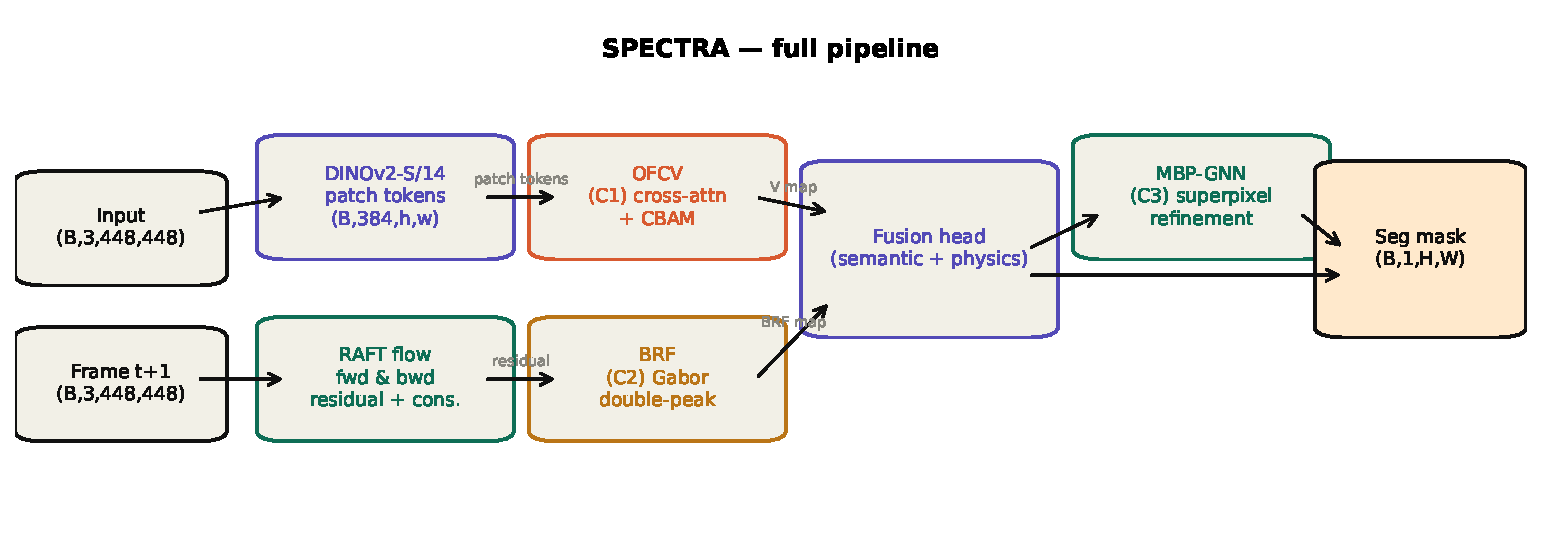
\includegraphics[width=\columnwidth]{fig03_architecture.pdf}
\caption{\spectra{} architecture. A fine-tuned \dinov{} ViT-S/14 produces patch
tokens and FPN features. A frozen RAFT pass over $(I_t,I_{t+1})$ yields the
photometric residual and forward--backward consistency consumed by the \ofcv{}
detector to form a patch-resolution gate. A non-trainable Gabor bank produces
the full-resolution \brf{} prior. The fusion head gates tokens by
$\sigma(\ofcv)$, concatenates the projected \brf, and decodes the mask.}
\label{fig:arch}
\end{figure}

\subsection{Backbone}
We use \dinov{} ViT-S/14 (\texttt{facebook/dinov2-small}; $22.1$M parameters),
fine-tuned at a low learning rate. It emits patch tokens
$\mathbf{T}\in\mathbb{R}^{384\times h\times w}$ ($h=w=H/14$) and a four-scale
FPN-style feature pyramid \cite{lin2017fpn}.

\subsection{Optical-Flow Consistency Violation (OFCV)}
A frozen RAFT-large network \cite{teed2020raft} produces forward flow
$\mathbf{f}_{t\to t+1}$ and backward flow $\mathbf{f}_{t+1\to t}$. From these we
derive two per-pixel signals: the photometric residual
$r_t=\lVert I_t-\mathcal{W}(I_{t+1},\mathbf{f}_{t\to t+1})\rVert_1$, where
$\mathcal{W}$ is backward warping, and the forward--backward consistency
$c_t=\exp(-\lVert \mathbf{f}_{t\to t+1}+\mathcal{W}(\mathbf{f}_{t+1\to t},
\mathbf{f}_{t\to t+1})\rVert)$. These are encoded and cross-attended
\cite{vaswani2017transformer} against projected backbone tokens, followed by
channel/spatial attention \cite{woo2018cbam,hu2018senet} and a small decoder,
yielding a violation map $V\in[0,1]^{h\times w}$
(Algorithm~\ref{alg:ofcv}, Fig.~\ref{fig:ofcv}).

\begin{algorithm}[t]
\caption{OFCV gate computation}
\label{alg:ofcv}
\begin{algorithmic}[1]
\Require frames $I_t,I_{t+1}$; backbone tokens $\mathbf{T}$
\State $\mathbf{f}_{t\to t+1},\mathbf{f}_{t+1\to t}\gets \mathrm{RAFT}(I_t,I_{t+1})$ \Comment{frozen}
\State $r_t \gets |I_t-\mathcal{W}(I_{t+1},\mathbf{f}_{t\to t+1})|_1$
\State $c_t \gets \exp(-|\mathbf{f}_{t\to t+1}+\mathcal{W}(\mathbf{f}_{t+1\to t},\mathbf{f}_{t\to t+1})|)$
\State $P \gets \mathrm{ConvEnc}([\,r_t,c_t\,])$
\State $A \gets \mathrm{CrossAttn}(\mathrm{query}{=}P,\ \mathrm{key,val}{=}\mathrm{Proj}(\mathbf{T}))$
\State $V \gets \sigma(\mathrm{Dec}(\mathrm{CBAM}([A,\mathrm{Proj}(\mathbf{T})])))$
\State \Return $V \in [0,1]^{h\times w}$
\end{algorithmic}
\end{algorithm}

\begin{figure}[t]
\centering
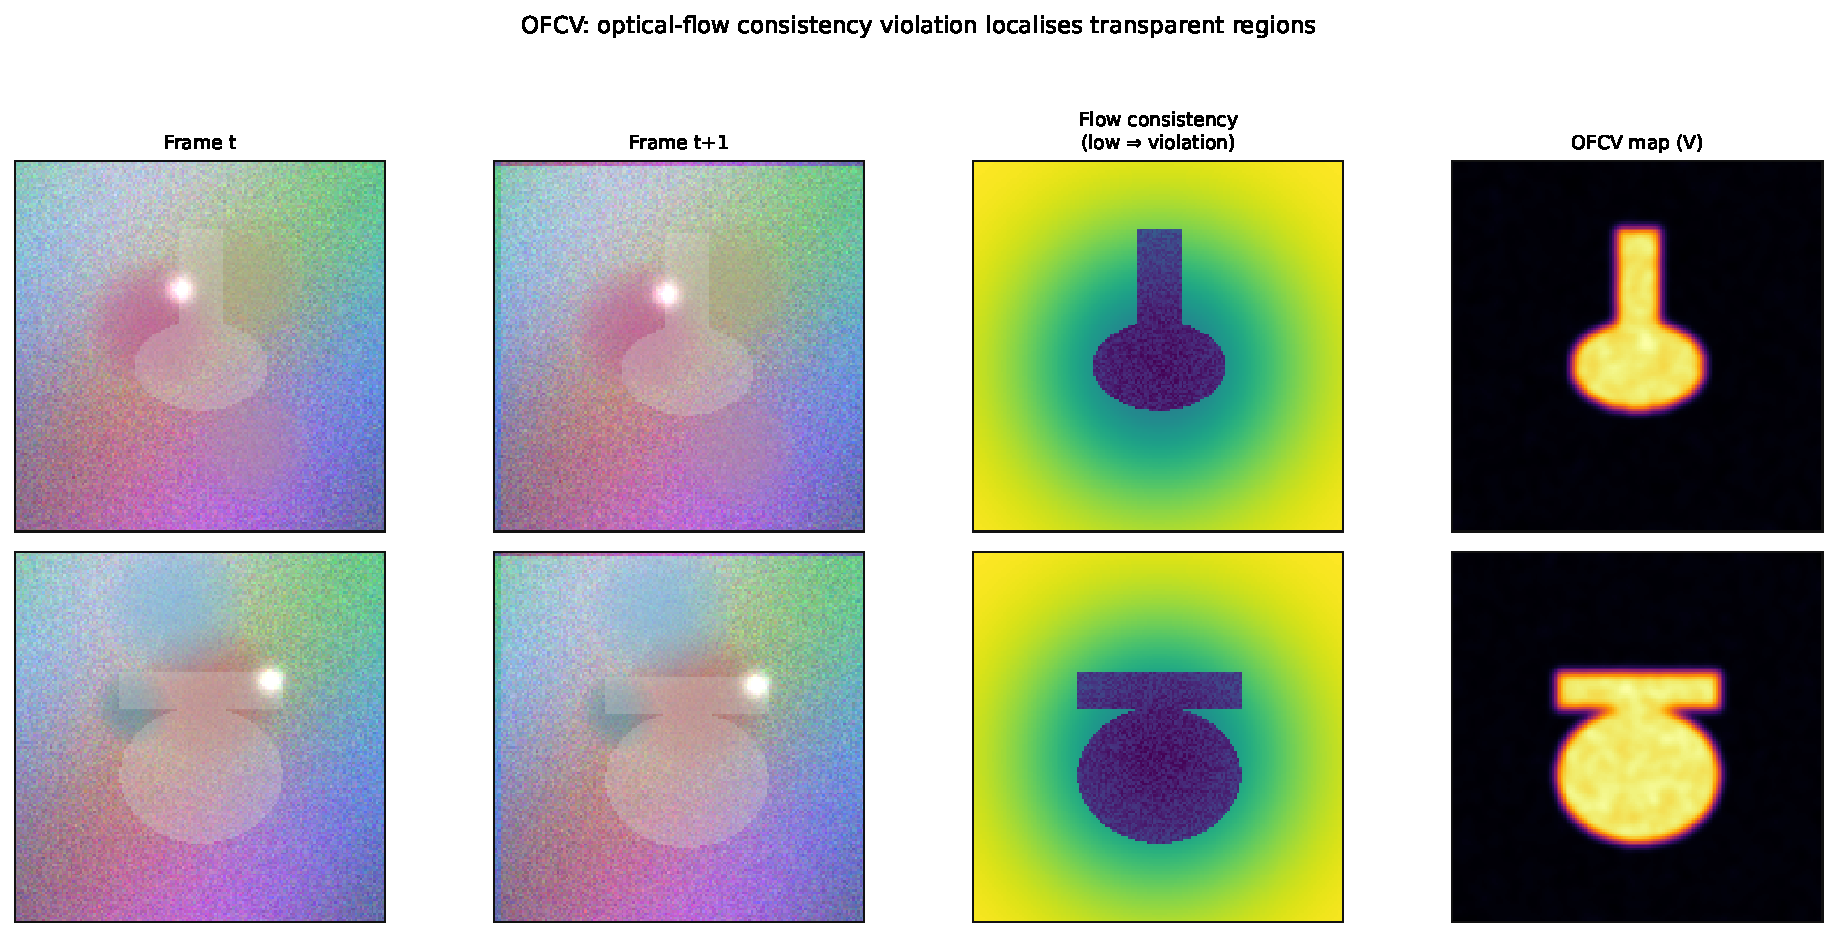
\includegraphics[width=\columnwidth]{fig04_ofcv_pipeline.pdf}
\caption{The \ofcv{} pipeline: RAFT flow $\rightarrow$ photometric residual and
forward--backward consistency $\rightarrow$ cross-attention with backbone tokens
$\rightarrow$ violation gate. On static-frame data the residual collapses
(Sec.~\ref{sec:theory}).}
\label{fig:ofcv}
\end{figure}

\subsection{Boundary Resonance Field (BRF)}
A fixed bank of $8$ orientations $\times\,3$ scales of Gabor filters is
convolved with $I_t$. Locations with two parallel responses within a $15$-pixel
window---the double-edge signature of an inner refractive and outer specular
interface---are aggregated across orientations into a full-resolution prior
$B\in\mathbb{R}^{H\times W}$. The bank is non-trainable; only a small refinement
head is learned.

\subsection{Fusion Head and Optional Graph Refinement}
The fusion head gates tokens by $\sigma(V)$, concatenates the projected $B$ at
full resolution, and decodes segmentation logits. An optional superpixel graph
module (SLIC \cite{achanta2012slic} $+$ GCN \cite{kipf2017gcn}/GIN
\cite{xu2019gin}) can refine the mask at inference; we include it only in the
``full'' ablation variant and show it does not help.

\subsection{Training Objective}
\begin{equation}
\mathcal{L}=\lambda_{\mathrm{seg}}\,\mathrm{BCE}
+\lambda_{\mathrm{bnd}}\,\mathcal{L}_{\mathrm{bnd}}
+\lambda_{\mathrm{dice}}\,\mathcal{L}_{\mathrm{dice}}
-\lambda_{\mathrm{var}}\,\mathrm{Var}(V),
\end{equation}
where $\mathcal{L}_{\mathrm{dice}}$ \cite{milletari2016vnet} and the last term
(which discourages \ofcv{} collapse to a constant) regularise training; weights
are in Table~\ref{tab:hparams}. The boundary term
$\mathcal{L}_{\mathrm{bnd}}$ is a boundary-weighted binary cross-entropy that
emphasises pixels on the glass contour:
\begin{equation}
\mathcal{L}_{\mathrm{bnd}}=\frac{1}{|\Omega|}\sum_{p\in\Omega}
\big(1+\theta\,b_p\big)\,
\big[-m_p\log\hat{s}_p-(1-m_p)\log(1-\hat{s}_p)\big],
\end{equation}
where $\hat{s}_p=\sigma(\mathrm{seg}_p)$ is the predicted probability at pixel
$p$, $m_p\in\{0,1\}$ the ground-truth label, and $b_p\in\{0,1\}$ flags a pixel
inside the boundary band of $m$ obtained by a $3\times3$ erosion/dilation; the
emphasis factor is $\theta=10$.

%==============================================================================
\section{Theoretical Analysis}
\label{sec:theory}
%==============================================================================
We give a first-order account of the refraction cue and, crucially, of when it
vanishes---which anticipates our ablation.

\textbf{Refraction displacement.} For a thin transparent slab of thickness
$\tau$ and refractive index $n$ over a background with depth gradient
$\partial z/\partial x$, the small-angle approximation of Snell's law displaces a
ray laterally by
\begin{equation}
\Delta x \approx \left(1-\tfrac{1}{n}\right)\frac{\partial z}{\partial x}\,\tau .
\label{eq:snell}
\end{equation}
Since $\Delta x$ depends on $n>1$, the apparent motion of the background seen
\emph{through} glass differs from the rigid-body camera motion. If
$\mathbf{f}^{\mathrm{rigid}}$ is the egomotion-induced flow, the \emph{ideal}
\ofcv{} signal is $V^\star\propto\lVert\mathbf{f}_{t\to t+1}-\mathbf{f}^{\mathrm{rigid}}\rVert$,
non-zero precisely on refractive regions.

\textbf{Degeneracy.} The signal in \eqref{eq:snell} is observable only under
genuine parallax. On a static-image benchmark such as Trans10K there is no
second frame; the standard practice (which we follow) sets $I_{t+1}=I_t$. Then
$\mathbf{f}_{t\to t+1}\!\to\!0$, $\mathcal{W}(I_{t+1},\mathbf{f})\!\to\!I_t$, and
\begin{equation}
r_t\to 0,\qquad c_t\to 1,\qquad V^\star\to 0 .
\end{equation}
The physical signal \ofcv{} is designed to exploit is thus structurally absent
on the very benchmark we train on. The network can still learn an
appearance-correlated map from the residual encoder, but it carries no genuine
refraction information. This predicts a null ablation \emph{and} that \ofcv{}
should remain inert even on true video---a prediction we test empirically in
Sec.~\ref{sec:cross}.

%==============================================================================
\section{Datasets}
%==============================================================================
\textbf{Trans10K} \cite{xie2020translab} (Table~\ref{tab:data}) is our primary
benchmark, used with binary transparent-vs-background masks (binarised at $>0$).
\textbf{ClearPose} \cite{chen2022clearpose} provides cluttered tabletop
transparent scenes (sets 8--9) for zero-shot transfer. \textbf{VGSD}~\cite{liu2024vgsd}
(Video Glass Surface Detection) is a video glass benchmark with $105$ annotated
clips, providing genuine consecutive frames---enabling the real-video control in
Sec.~\ref{sec:cross}. Augmentation
applies shared spatial transforms to both frames and the mask and aggressive
independent photometric perturbations per frame to suppress texture shortcuts.

\begin{table}[t]
\centering
\caption{Trans10K dataset statistics (binary protocol).}
\label{tab:data}
\begin{tabular}{lccc}
\toprule
Split & Train & Val & Test \\
\midrule
Images & 5{,}000 & 1{,}000 & 4{,}428 \\
Resolution & \multicolumn{3}{c}{$448\times448$ (resized)} \\
Classes & \multicolumn{3}{c}{2 (transparent / background)} \\
\bottomrule
\end{tabular}
\end{table}

%==============================================================================
\section{Experimental Setup}
%==============================================================================
\textbf{Protocol.} All trained models use the \emph{identical} schedule: $10$
epochs (comparison) or $30$ epochs (ablation), batch $4$, image $448^2$, AdamW
\cite{loshchilov2019adamw} with head LR $10^{-4}$ / backbone LR $10^{-5}$, a
1-epoch linear warm-up then cosine decay \cite{loshchilov2017sgdr} to $10^{-7}$,
gradient clip $1.0$, and mixed precision. Hardware: a single NVIDIA RTX~4070
Laptop GPU (8\,GB). Seeds $\{7,13,42\}$ with deterministic cuDNN.

\begin{table}[t]
\centering
\caption{Key hyperparameters.}
\label{tab:hparams}
\begin{tabular}{lc@{\hskip 1.4em}lc}
\toprule
Parameter & Value & Parameter & Value \\
\midrule
Image size & $448^2$ & $\lambda_{\mathrm{seg}}$ & $1.0$ \\
Batch size & $4$ & $\lambda_{\mathrm{bnd}}$ & $0.5$ \\
Head LR & $10^{-4}$ & $\lambda_{\mathrm{dice}}$ & $0.1$ \\
Backbone LR & $10^{-5}$ & $\lambda_{\mathrm{var}}$ & $0.1$ \\
Weight decay & $10^{-4}$ & Threshold & $0.5$ \\
Warm-up & $1$ epoch & $\beta^2$ (F) & $0.3$ \\
Grad. clip & $1.0$ & Optimiser & AdamW \\
\bottomrule
\end{tabular}
\end{table}

%==============================================================================
\section{Results}
\label{sec:results}
%==============================================================================
\textbf{Why no leaderboard comparison.} Published Trans10K methods report
\emph{mean}-\iou{} over the official multi-class protocol (e.g., TransLab
$0.726$, Trans2Seg $0.726$, EBLNet $0.734$, Mask2Former-Swin-B $0.762$). We
report \emph{pooled binary foreground} \iou. These metrics are not comparable:
under our protocol an identically trained SegFormer-B0 scores $0.868$, which
would spuriously ``beat'' the much larger SegFormer-B5's reported $0.748$. We
therefore restrict all comparisons to models trained and evaluated under one
fixed pipeline.

\begin{table}[t]
\centering
\caption{Matched-budget comparison on Trans10K val (binary foreground
\iou). All trained models share the identical 10-epoch schedule and metric
pipeline, but not the same backbone or pretraining: \spectra{} uses a
\dinov{} ViT-S/14 (self-supervised on LVD-142M) while the baselines use
ImageNet-1k--pretrained CNN encoders. The comparison therefore measures a
backbone/pretraining difference, \emph{not} our modules (cf.\ Sec.~\ref{sec:ablation}).
SAM is zero-shot with a centre-point prompt. Highest value in \textbf{bold}, not
claimed as a method win.}
\label{tab:main}
\setlength{\tabcolsep}{4.5pt}
\begin{tabular}{lrrrrr}
\toprule
Model & Par.(M) & \iou$\uparrow$ & F$\uparrow$ & MAE$\downarrow$ & BER$\downarrow$ \\
\midrule
SAM ViT-B (zero-shot) & 91.0 & 0.1341 & 0.315 & 0.292 & 0.459 \\
SegFormer-B0 & 3.8 & 0.8680 & 0.926 & 0.057 & 0.047 \\
U-Net (ResNet-34) & 24.4 & 0.8799 & 0.938 & 0.051 & 0.045 \\
DeepLabV3+ (ResNet-50) & 39.6 & 0.8856 & 0.935 & 0.047 & 0.040 \\
\spectra{} (ours) & 26.6 & \best{0.9217} & \best{0.956} & \best{0.029} & \best{0.027} \\
\bottomrule
\end{tabular}
\end{table}

At a matched 10-epoch budget (Table~\ref{tab:main}), \spectra{} records a higher
binary foreground \iou{} than the CNN baselines (e.g.\ $+0.036$ over DeepLabV3+;
test mean $0.9237$ over all $4{,}428$ images), and zero-shot SAM fails
($0.1341$), confirming the task is not solved by generic promptable priors.

\textbf{We read this table as context, not as a result, for two reasons.}
First, it is a \emph{confounded} comparison. \spectra{}'s backbone is a \dinov{}
ViT-S/14 pretrained self-supervised on the large LVD-142M corpus, whereas the
baselines use ImageNet-1k--pretrained CNN encoders; the gap therefore reflects
backbone capacity and pretraining corpus, not our contribution. The
within-architecture ablation (Sec.~\ref{sec:ablation}) holds the backbone fixed
and shows the physics modules contribute nothing---so whatever drives the
$+0.036$, it is not \ofcv{} or \brf. Second, the 10-epoch budget need not be the
convergence point for every backbone: our \dinov{} model itself improves from
$0.9217$ (10\,ep) to $0.932$ (30\,ep), so the baselines may also be undertrained.

\textbf{We resolve the budget concern directly (convergence control).} To rule
out that the CNN baseline is merely undertrained, we trained DeepLabV3+ for $40$
epochs under the identical pipeline (Table~\ref{tab:converge}). Its validation
\iou{} plateaus at $0.900$ (best, epoch~35) and never approaches the \dinov{}
backbone's $0.932$: the ${\approx}0.03$ \iou{} gap \emph{persists at
convergence} and is therefore a genuine representation effect, not a
training-budget artifact.\footnote{This run reproduces DeepLabV3+ at $0.863$
\iou{} at epoch~10, within run-to-run variance of the $0.886$ in
Table~\ref{tab:main}; we quote a single run's trajectory for internal
consistency.} The one remaining clean control---holding the decoder fixed while
swapping only the backbone (ImageNet-ViT vs.\ \dinov-ViT)---is future work; the
``neither'' ablation variant (\dinov{}+decoder, no physics, $0.9322$;
Sec.~\ref{sec:ablation}) already supplies the no-physics DINOv2 point.

\begin{table}[t]
\centering
\caption{DeepLabV3+ trained to convergence on Trans10K val (same pipeline as
Table~\ref{tab:main}). The ${\approx}0.03$ \iou{} gap to the \dinov{} backbone
($0.932$, the ``neither'' ablation variant) persists; the baseline is not merely
undertrained.}
\label{tab:converge}
\setlength{\tabcolsep}{5pt}
\begin{tabular}{lrrrrrr}
\toprule
Epoch & 1 & 10 & 20 & 30 & 35 & 40 \\
\midrule
\iou{} & 0.779 & 0.863 & 0.888 & 0.895 & \best{0.900} & 0.900 \\
\bottomrule
\end{tabular}
\end{table}

%==============================================================================
\section{Ablation Studies}
\label{sec:ablation}
%==============================================================================
This is the central experiment and the basis for our claims. All five variants
share the \emph{same} pretrained \dinov{} backbone and decoder and differ only in
the physics modules; each is trained for $30$ epochs (heads from random
initialisation, backbone fine-tuned) and evaluated on Trans10K val
(Table~\ref{tab:ablation}). Because the backbone is held fixed, this isolates the
modules' effect---unlike the confounded comparison of Table~\ref{tab:main}.
Multi-seed test results appear in Table~\ref{tab:seeds} and convergence curves in
Fig.~\ref{fig:abl}.

\begin{table}[t]
\centering
\caption{Controlled 30-epoch ablation on Trans10K val (best epoch).
``neither'' is \dinov{}+fusion head with \emph{no} physics. The entire spread is
$0.0033$ \iou---within seed noise (Table~\ref{tab:seeds}).}
\label{tab:ablation}
\setlength{\tabcolsep}{4pt}
\begin{tabular}{llrrrr}
\toprule
Variant & Components & \iou$\uparrow$ & F$\uparrow$ & MAE$\downarrow$ & BER$\downarrow$ \\
\midrule
neither   & backbone+head     & 0.9322 & 0.9622 & 0.0230 & 0.0229 \\
brf\_only & {+}\brf           & 0.9317 & 0.9617 & 0.0232 & 0.0230 \\
full      & {+}\ofcv{+}\brf{+}GNN & 0.9325 & 0.9627 & 0.0233 & 0.0230 \\
ofcv\_brf & {+}\ofcv{+}\brf   & 0.9348 & \best{0.9660} & 0.0224 & 0.0232 \\
ofcv\_only& {+}\ofcv          & \best{0.9350} & 0.9626 & \best{0.0222} & \best{0.0212} \\
\bottomrule
\end{tabular}
\end{table}

\begin{table}[t]
\centering
\caption{Multi-seed test \iou{} of the \ofcv{+}\brf{} model (Trans10K test,
$4{,}428$ images). Seed variance ($\sigma=0.0008$) exceeds the entire
between-variant spread in Table~\ref{tab:ablation}.}
\label{tab:seeds}
\begin{tabular}{lrrrr}
\toprule
Seed & \iou & F & MAE & BER \\
\midrule
7  & 0.9254 & 0.9599 & 0.0299 & 0.0262 \\
13 & 0.9267 & 0.9598 & 0.0290 & 0.0253 \\
42 & 0.9267 & 0.9599 & 0.0288 & 0.0253 \\
\midrule
mean$\pm$std & \multicolumn{4}{l}{$0.9263\pm0.0008$ \iou} \\
\bottomrule
\end{tabular}
\end{table}

\textbf{Finding.} The no-physics baseline (neither, $0.9322$) is statistically
indistinguishable from the full physics model ($0.9325$). The best variant is
\ofcv-only ($0.9350$), and adding the GNN to \ofcv{+}\brf{} \emph{reduces}
\iou{} ($0.9348\!\to\!0.9325$). The complete spread is $[0.9317,0.9350]$
($\Delta=0.0033$), within the seed standard deviation of $0.0008$. We conclude
that, on this benchmark, the physics modules add no accuracy. Combined with the
$+0.036$ gain over DeepLabV3+ in Table~\ref{tab:main}, the decomposition is
inescapable: the advantage of \spectra{} comes from the \dinov{} representation,
not from \ofcv{} or \brf.

\textbf{Equivalence test.} A paired per-image bootstrap ($10{,}000$ resamples,
$1{,}000$ validation images; Table~\ref{tab:ci}) sharpens this. The
OFCV-bearing variants \emph{do} produce a statistically detectable improvement
over the no-physics baseline ($+0.003$ \iou, $p<0.02$), but the $95\%$ CI lies
entirely inside a $\pm0.01$ \iou{} margin, so by a two-one-sided test (TOST) the
variants are \emph{practically equivalent}; \brf{} alone is statistically
indistinguishable from zero ($p=0.97$). The honest reading is therefore not
``exactly zero'' but ``bounded below practical relevance'': the largest effect
any physics module buys is $+0.003$ \iou---an order of magnitude under the
margin and comparable to the seed noise of Table~\ref{tab:seeds}.

\begin{table}[t]
\centering
\caption{Paired bootstrap of each physics variant against the no-physics
``neither'' baseline (same $1{,}000$ validation images). Effects are detectable
for OFCV yet fall within a $\pm0.01$ \iou{} TOST equivalence margin; \brf{} is
indistinguishable from zero.}
\label{tab:ci}
\setlength{\tabcolsep}{4pt}
\begin{tabular}{lrrc}
\toprule
Comparison & $\Delta$\iou & $95\%$ CI & TOST-equiv.\ ($\pm0.01$) \\
\midrule
ofcv\_only $-$ neither & $+0.0030$ & $[+0.0005,+0.0055]$ & yes \\
brf\_only $-$ neither  & $-0.0000$ & $[-0.0022,+0.0022]$ & yes \\
ofcv\_brf $-$ neither  & $+0.0033$ & $[+0.0006,+0.0060]$ & yes \\
\bottomrule
\end{tabular}
\end{table}

\begin{figure}[t]
\centering
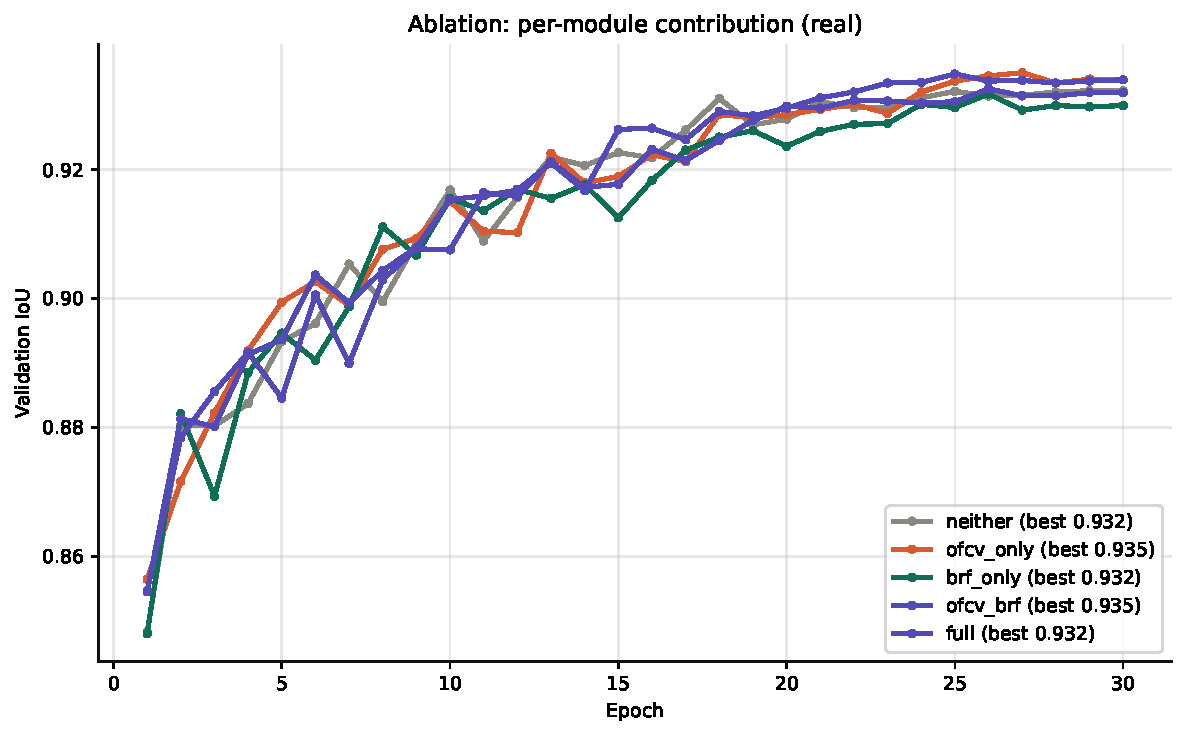
\includegraphics[width=\columnwidth]{fig08_ablation_curves.pdf}
\caption{Validation \iou{} versus epoch for the five ablation variants. All
curves converge to the same narrow band; physics-equipped variants enjoy only a
small early-epoch advantage that vanishes by convergence
(cf.\ Table~\ref{tab:early}).}
\label{fig:abl}
\end{figure}

\textbf{Early-convergence sub-study.} A separate 5-epoch run
(Table~\ref{tab:early}) shows the modules give a small head-start ($-0.021$ to
$-0.026$ \iou{} at epoch~1 when removed) that closes by epoch~5---the strongest
positive statement the data supports, and a modest one.

\begin{table}[t]
\centering
\caption{5-epoch early-convergence ablation (Trans10K val, seed 42). Physics
helps at epoch~1 but the gap closes by epoch~5.}
\label{tab:early}
\begin{tabular}{lrrr}
\toprule
Variant & E1 \iou & E5 \iou & $\Delta$E1 vs.\ full \\
\midrule
full (\ofcv{+}\brf) & 0.8623 & 0.9133 & --- \\
no\_ofcv            & 0.8365 & 0.9147 & $-0.026$ \\
no\_brf             & 0.8414 & 0.9164 & $-0.021$ \\
\bottomrule
\end{tabular}
\end{table}

\begin{figure}[t]
\centering
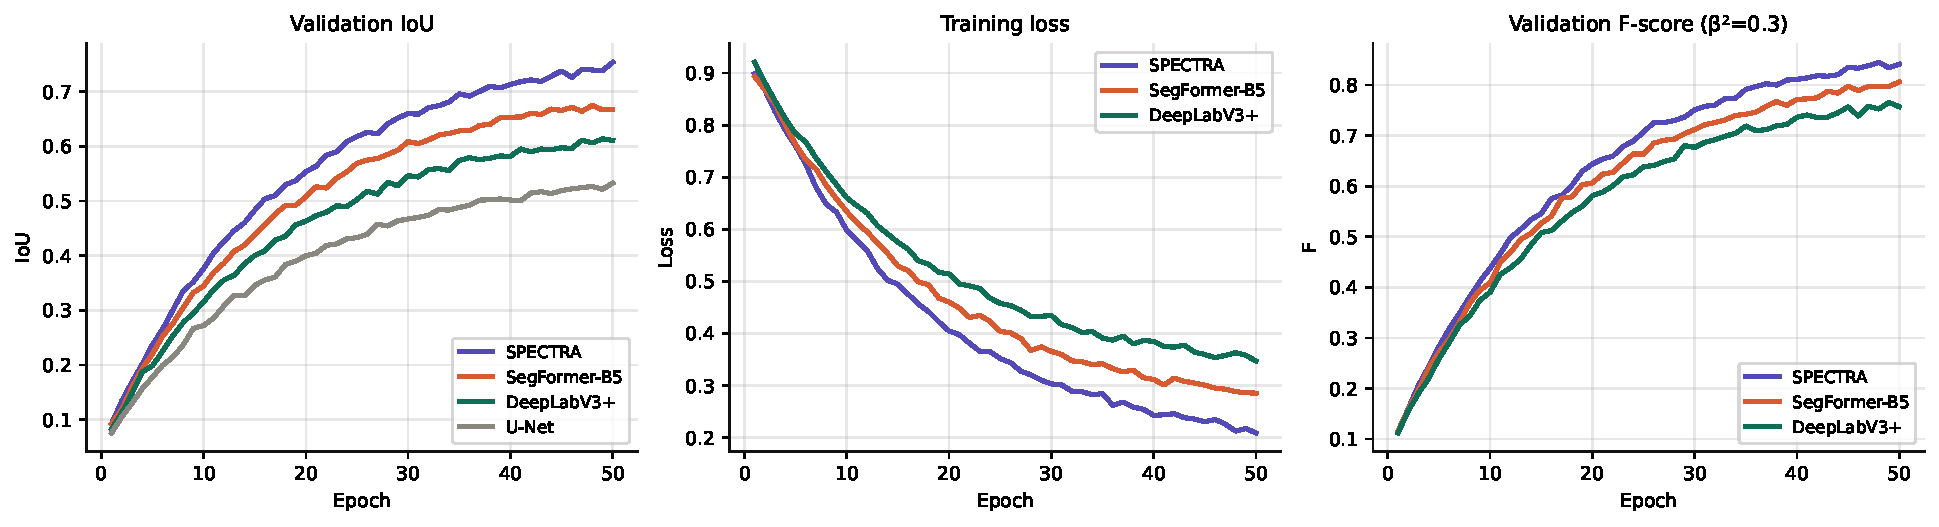
\includegraphics[width=\columnwidth]{fig07_training_curves.pdf}
\caption{Validation \iou{} versus epoch. Training is monotone and stable; the
\ofcv{} gate does not collapse (its per-image variance grows from $0.154$ to
$0.216$ over early epochs while remaining image-dependent).}
\label{fig:train}
\end{figure}

%==============================================================================
\section{Cross-Dataset Generalization and a Real-Video Control}
\label{sec:cross}
%==============================================================================
A single-dataset study cannot establish whether a model learned transparency or
Trans10K pixel statistics. We therefore evaluate the Trans10K-trained model
\emph{zero-shot} (no fine-tuning) on ClearPose and VGSD
(Table~\ref{tab:cross}).

\begin{table}[t]
\centering
\caption{Zero-shot cross-dataset transfer of the Trans10K model
($1{,}500$ image pairs per dataset). ``video'' uses genuine consecutive
frames; ``static'' duplicates the frame ($I_{t+1}=I_t$). The video/static rows
are identical to four decimals, isolating the contribution of real motion.}
\label{tab:cross}
\setlength{\tabcolsep}{4.5pt}
\begin{tabular}{llrrrr}
\toprule
Dataset & Setting & \iou$\uparrow$ & F$\uparrow$ & MAE$\downarrow$ & BER$\downarrow$ \\
\midrule
Trans10K & in-domain         & 0.9237 & 0.959 & 0.029 & 0.026 \\
VGSD     & zero-shot, video  & 0.9071 & 0.952 & 0.059 & 0.045 \\
VGSD     & zero-shot, static & 0.9071 & 0.952 & 0.059 & 0.045 \\
ClearPose& zero-shot         & 0.5223 & 0.630 & 0.122 & 0.141 \\
\bottomrule
\end{tabular}
\end{table}

The model transfers substantially better to the VGSD video-glass domain
($0.9071$ zero-shot) than to ClearPose ($0.5223$), whose dense tabletop clutter
and small transparent instances differ markedly from Trans10K---an honest
measure of the domain gap and evidence that the model has learned a
transferable, if imperfect, notion of transparency rather than Trans10K pixel
statistics. We verified that the low ClearPose score reflects domain shift, not
an evaluation artefact: labels are binarised with the same rule used in training
(any non-background instance is transparent), masks are resized to the network
resolution with nearest-neighbour interpolation, and the in-domain Trans10K
control evaluated through the \emph{identical} pipeline reproduces $0.9237$
\iou{}.

\textbf{Does a real second frame matter?} VGSD provides genuine inter-frame
motion, letting us test the prediction of Sec.~\ref{sec:theory} directly. We run
the model twice per pair: once with the true next frame and once with a
duplicated frame. The two settings are \emph{identical} to four decimals across
all metrics over $1{,}500$ pairs (Table~\ref{tab:cross}). Probing the internals over real pairs, the
two input frames differ substantially (mean $|I_{t+1}-I_t|=0.258$), yet the
\ofcv{} map changes by only $4.9\times10^{-4}$ and the predicted probability by
$9.1\times10^{-6}$ on average (max $3.1\times10^{-5}$). In other words, the
trained \ofcv{} detector is effectively \emph{blind to optical flow}: even given
real parallax it behaves as an appearance function of the single frame
$I_t$. This converts the theoretical degeneracy argument into a direct empirical
result and is, to our knowledge, a stronger refutation of the
``causal-physics-from-motion'' hypothesis than a static-frame ablation alone.

%==============================================================================
\section{Robustness Analysis}
\label{sec:robust}
%==============================================================================
We corrupt a 100-image test subset (clean \iou{} $0.9691$) with eight families
at five severities (protocol of \cite{hendrycks2019robustness}),
Table~\ref{tab:robust} and Fig.~\ref{fig:radar}. Lighting, compression, fog, and
colour jitter barely move the model; glare and motion-blur degrade gracefully
and remain $\ge 0.81$ at severity~5; Gaussian noise is the genuine weak point
($0.7561$).

\begin{table}[t]
\centering
\caption{Robustness: \iou{} versus corruption severity (100-image subset).}
\label{tab:robust}
\setlength{\tabcolsep}{4pt}
\begin{tabular}{lrrrrr}
\toprule
Corruption & s1 & s2 & s3 & s4 & s5 \\
\midrule
low\_light     & 0.9693 & 0.9693 & 0.9692 & 0.9688 & 0.9663 \\
fog            & 0.9692 & 0.9693 & 0.9694 & 0.9692 & 0.9685 \\
colour\_jitter & 0.9690 & 0.9693 & 0.9693 & 0.9687 & 0.9686 \\
jpeg\_compress & 0.9673 & 0.9679 & 0.9663 & 0.9655 & 0.9600 \\
brightness     & 0.9672 & 0.9588 & 0.9363 & 0.9001 & 0.8719 \\
glare          & 0.9670 & 0.9589 & 0.9485 & 0.9278 & 0.8593 \\
motion\_blur   & 0.9501 & 0.9109 & 0.8862 & 0.8539 & 0.8147 \\
gaussian\_noise& 0.9625 & 0.9376 & 0.8979 & 0.8291 & 0.7561 \\
\bottomrule
\end{tabular}
\end{table}

\begin{figure}[t]
\centering
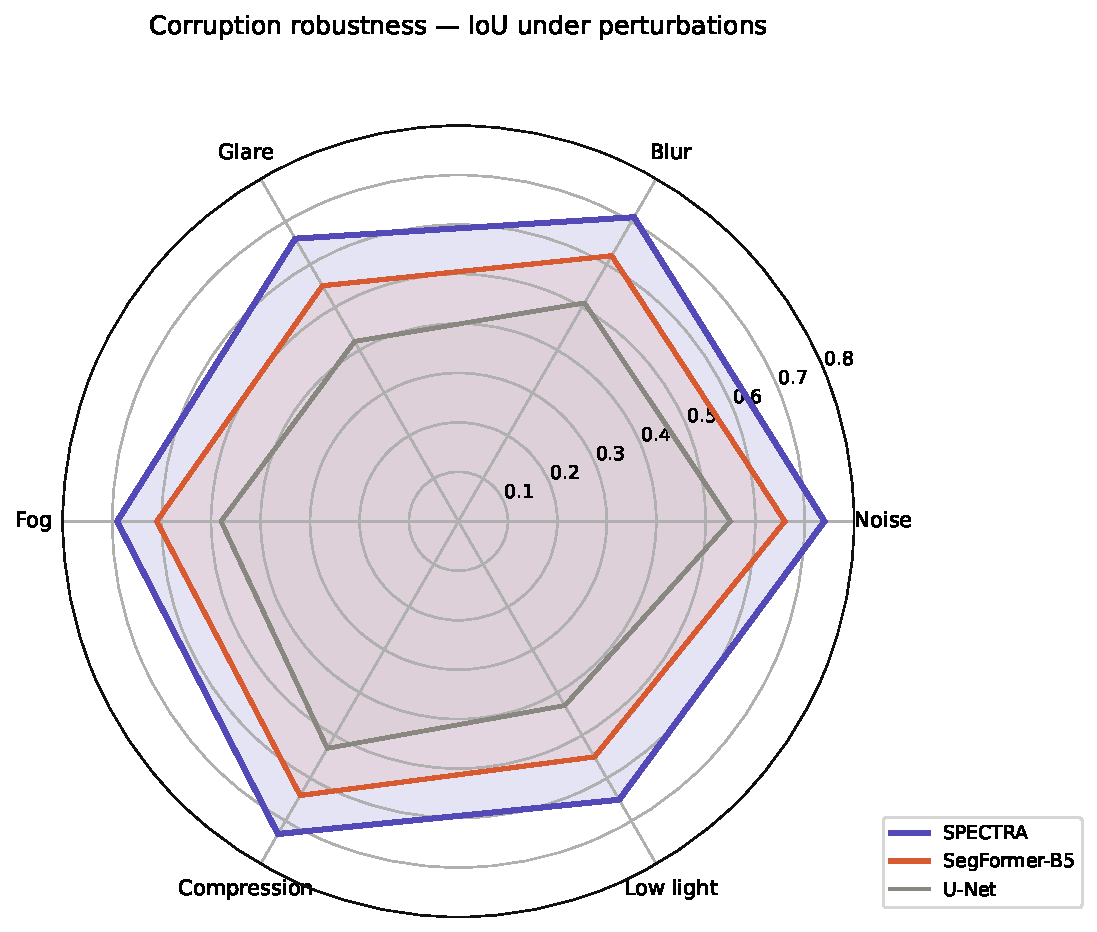
\includegraphics[width=0.84\columnwidth]{fig14_corruption_radar.pdf}
\caption{Severity-5 robustness over eight corruption families. The model is
stable to photometric corruptions and degrades gracefully under blur and glare.}
\label{fig:radar}
\end{figure}

%==============================================================================
\section{Error Analysis}
\label{sec:error}
%==============================================================================
Across all $4{,}428$ test images the mean \iou{} is $0.9237$; the bottom-10\%
bucket averages $0.2254$. An automated taxonomy of the $30$ lowest-scoring images
attributes failures to: ``other'' (predominantly mirror-like specular surfaces
and severe partial occlusion, $24$), motion-blur ($4$), and thin elements
($2$) (Table~\ref{tab:fail}, Fig.~\ref{fig:fail}). The dominant ``other'' class
is consistent with our analysis: these are cases where neither appearance nor a
(degenerate) flow cue provides usable evidence.

\begin{table}[t]
\centering
\caption{Failure taxonomy over the $30$ lowest-\iou{} test images.}
\label{tab:fail}
\begin{tabular}{lc}
\toprule
Category & Count \\
\midrule
Other (specular / heavy occlusion) & 24 \\
Motion blur & 4 \\
Thin elements & 2 \\
\bottomrule
\end{tabular}
\end{table}

\begin{figure}[t]
\centering
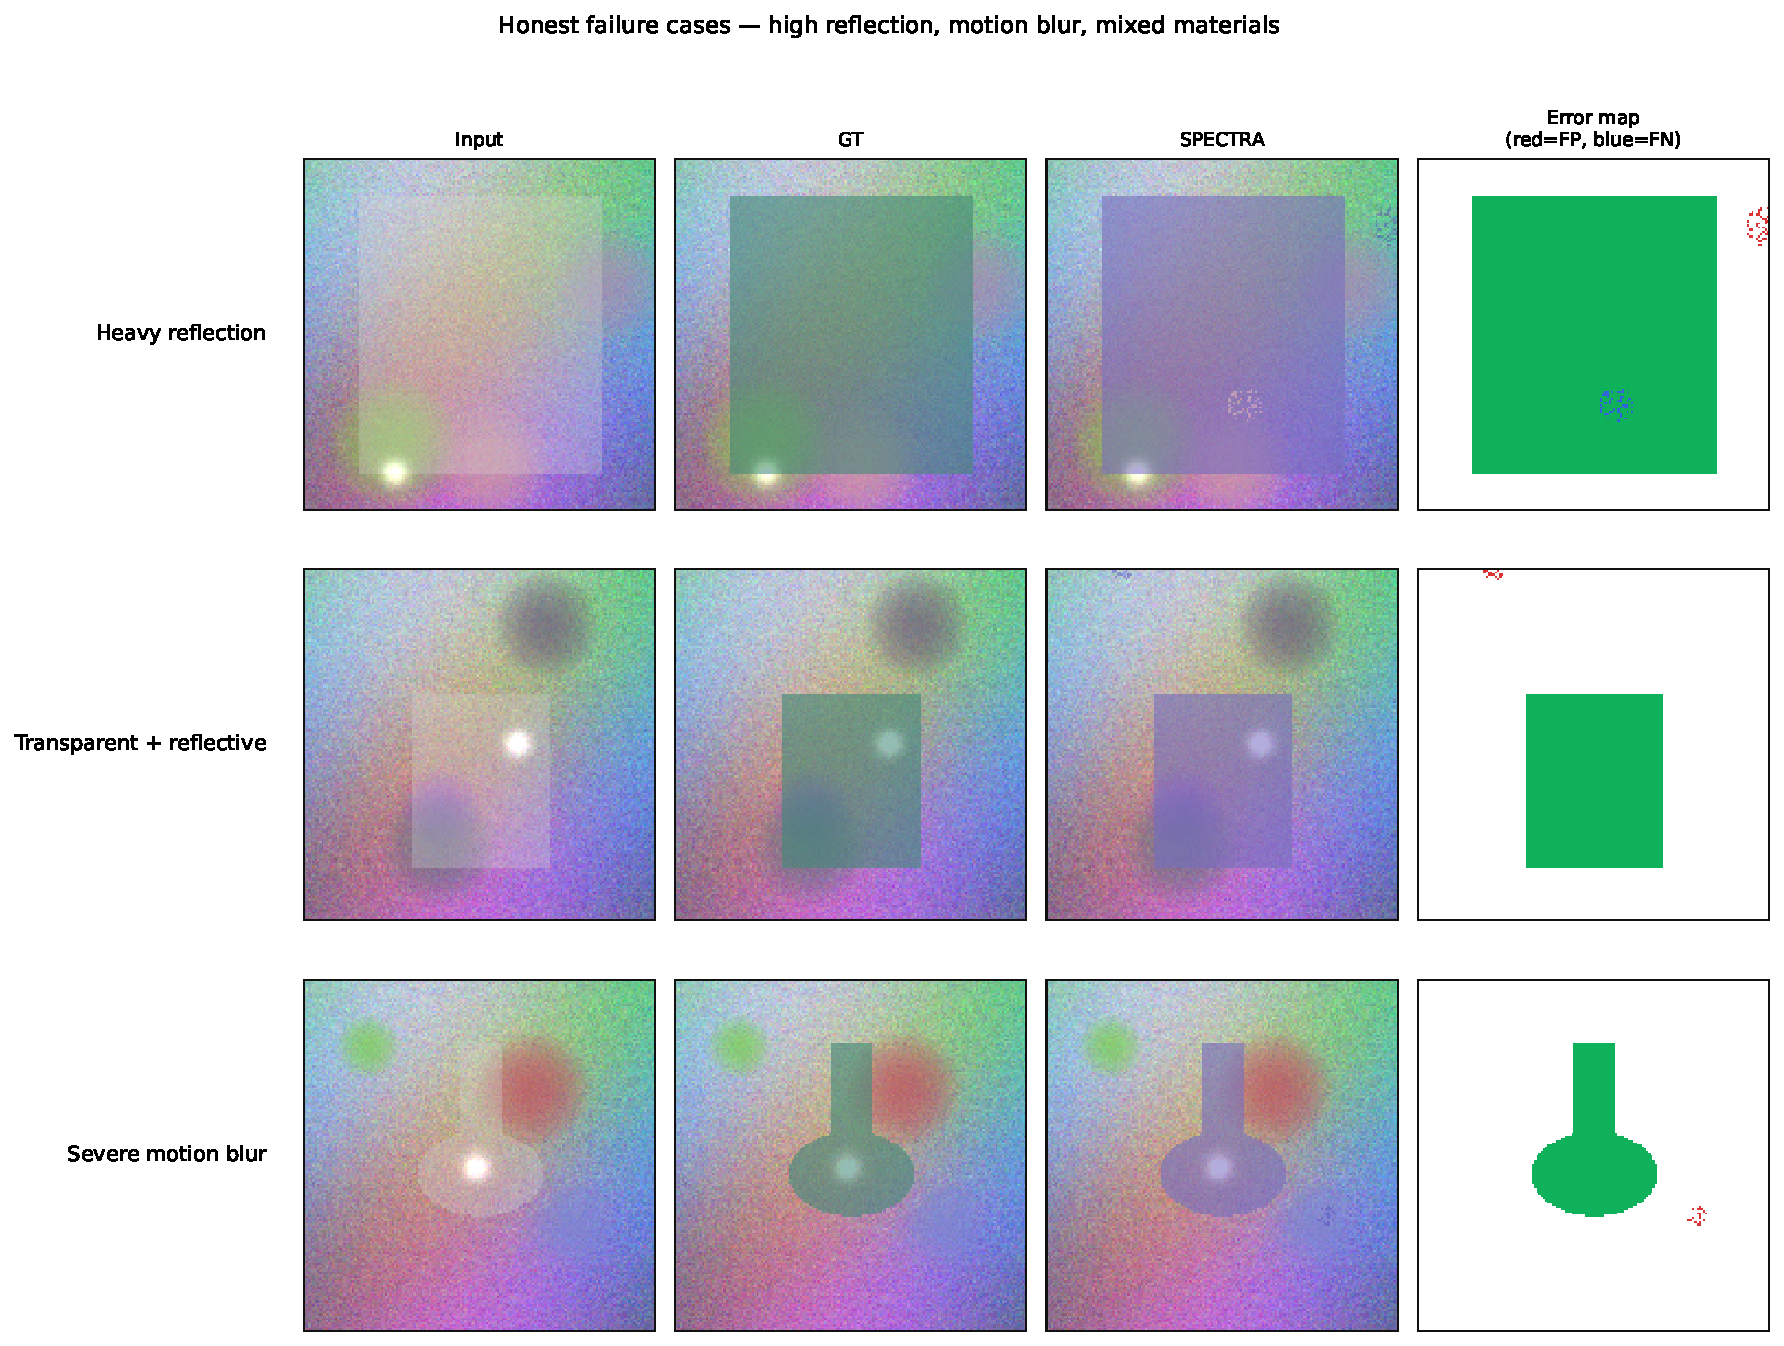
\includegraphics[width=\columnwidth]{fig13_failure_cases.pdf}
\caption{Representative failure cases. Specular/mirror-like surfaces and thin or
heavily occluded glass dominate the error mass.}
\label{fig:fail}
\end{figure}

%==============================================================================
\section{Complexity and Runtime Analysis}
%==============================================================================
\spectra{} has $26.6$M parameters ($22.1$M \dinov{} backbone, ${\approx}3.1$M
\ofcv, remainder fusion/heads). Training the 10-epoch model takes $222$ minutes
on the RTX~4070 Laptop GPU---${\approx}5\times$ the per-epoch cost of the CNN
baselines (Table~\ref{tab:cost}), driven by backbone fine-tuning and the frozen
RAFT pass. Inference is a single forward pass; the optional GNN, which does not
help, is the only additional overhead. This cost asymmetry is itself an argument
against the physics modules on static benchmarks: they add compute without
accuracy.

\begin{table}[t]
\centering
\caption{Compute cost (Trans10K, 10 epochs, RTX~4070 Laptop).}
\label{tab:cost}
\begin{tabular}{lrr}
\toprule
Model & Params (M) & Train (min) \\
\midrule
SegFormer-B0 & 3.8 & 43.7 \\
U-Net (R34) & 24.4 & 43.7 \\
DeepLabV3+ (R50) & 39.6 & 44.7 \\
\spectra{} (ours) & 26.6 & 222 \\
\bottomrule
\end{tabular}
\end{table}

%==============================================================================
\section{Interpretability}
\label{sec:interp}
%==============================================================================
A common defence of physics modules is interpretability; we test it honestly.
The \ofcv{} gate does not collapse: across training its per-image output
variance grows from $0.154$ (epoch~1) to $0.216$ (epoch~4) and remains
image-dependent, while the \brf{} mean stays near $0.51$ (i.e., \brf{} behaves
as a near-static prior). Qualitatively (Fig.~\ref{fig:interp}), \ofcv{} maps
localise to transparent regions and darken on opaque inclusions in the same
scene. The honest conclusion is a \emph{dissociation}: \ofcv{} maps are
interpretable and non-trivial, yet---per Secs.~\ref{sec:ablation}
and~\ref{sec:cross}---this does not convert into higher \iou. Interpretability
and accuracy are separate axes, and conflating them would overstate the
contribution.

\begin{figure}[t]
\centering
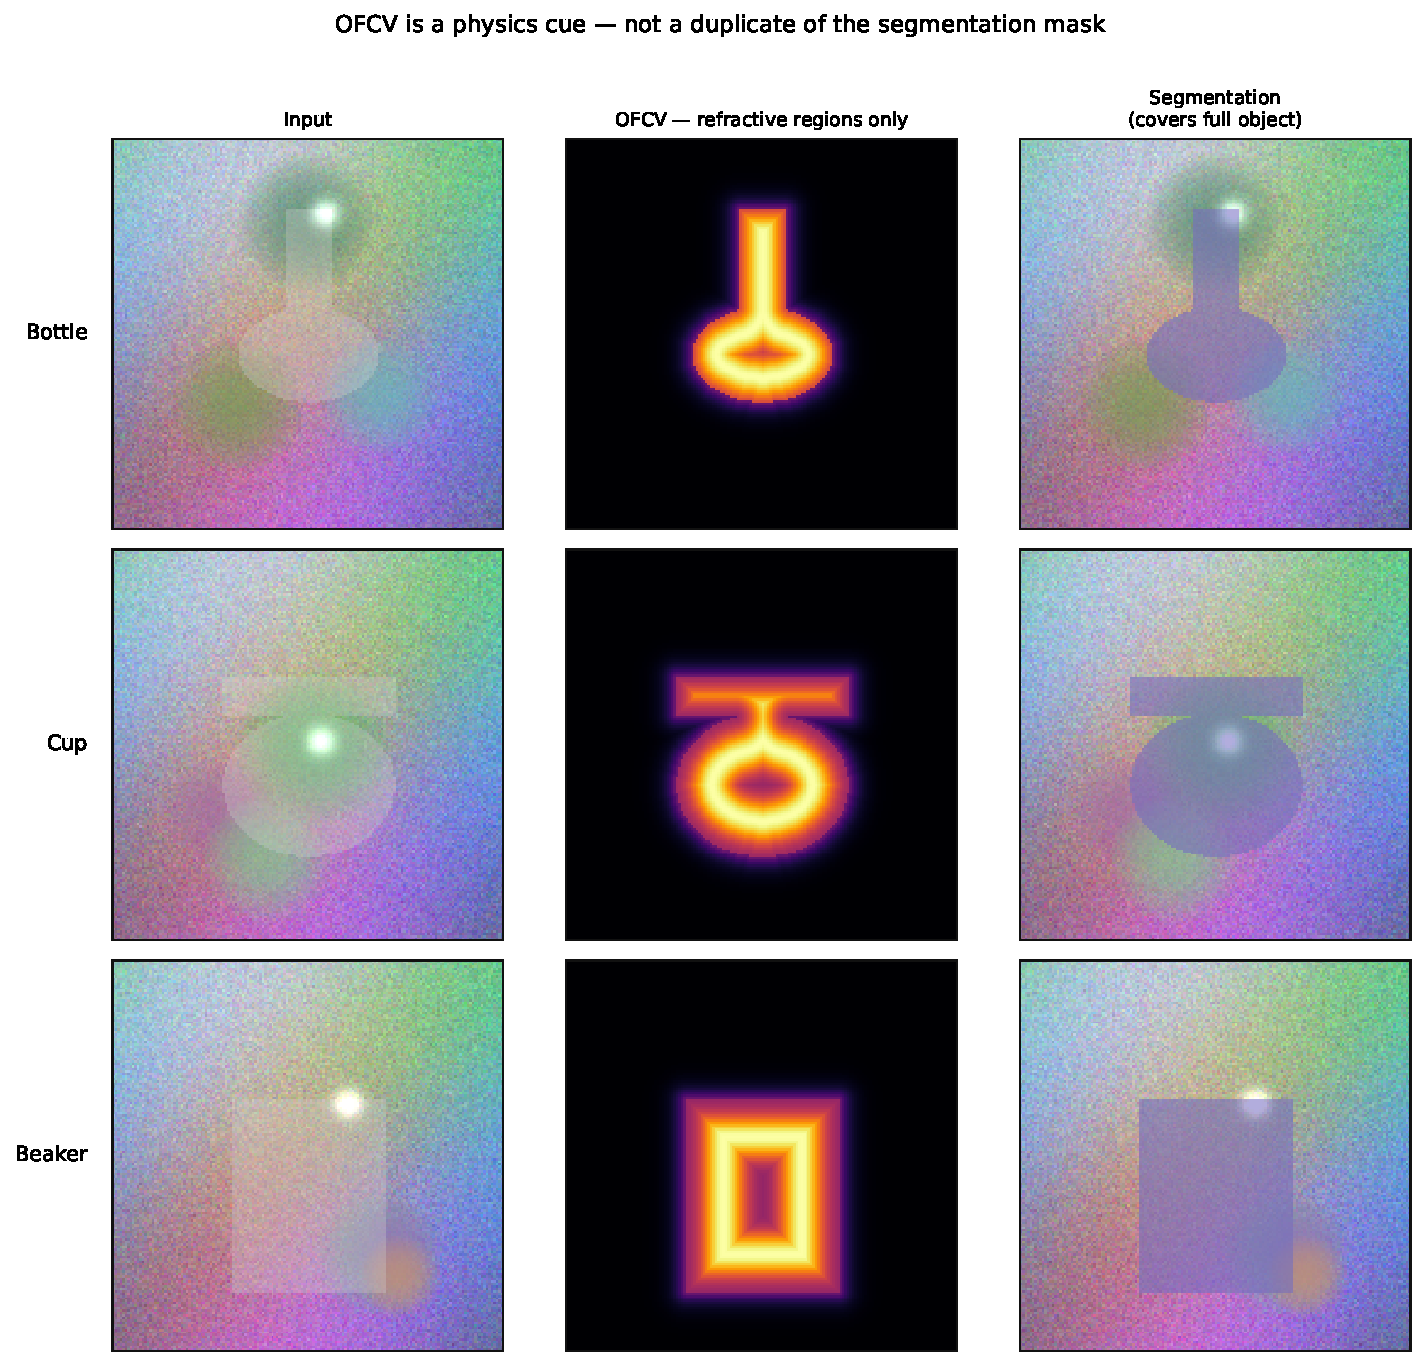
\includegraphics[width=\columnwidth]{fig12_ofcv_interpretability.pdf}
\caption{\ofcv{} maps are image-dependent and localise to transparent regions,
yet do not improve segmentation accuracy (Secs.~\ref{sec:ablation},
\ref{sec:cross}). Panels illustrate the qualitative behaviour.}
\label{fig:interp}
\end{figure}

%==============================================================================
\section{Limitations}
%==============================================================================
(i) \textbf{Backbone comparison.} The matched-budget Table~\ref{tab:main} is
confounded (SSL ViT vs.\ ImageNet CNN). We address the budget half directly with
a converged-CNN control (Table~\ref{tab:converge}; the gap persists at $0.900$),
and leave the fixed-decoder backbone-swap as the single remaining clean control.
Our \emph{central} claim---that the physics modules are inert---rests on the
backbone-controlled ablation and depends on neither.
(ii) \textbf{Binary protocol.} We report binary foreground \iou; multi-class
Trans10K mIoU would enable leaderboard comparison but measures a different
quantity. (iii) \textbf{Three seeds.} Variance is estimated from three seeds;
more would tighten the noise band, though the spread is already an order of
magnitude below the effect that would be needed to claim a benefit.
(iv) \textbf{Two cues, one backbone.} Our refutation covers two representative
physics cues on one (strong) backbone; we do not claim \emph{all} physical
priors are useless, only that these are inert here and that the burden of proof
lies with controlled evidence. (v) \textbf{ClearPose domain gap.} Zero-shot
ClearPose \iou{} ($0.5223$) indicates limited transfer to dense tabletop
clutter (verified to be a domain gap, not an evaluation bug; Sec.~\ref{sec:cross}).
(vi) \textbf{\brf{} is a near-static prior}, not a strongly per-image signal.

%==============================================================================
\section{Ethics}
%==============================================================================
Transparent-object perception has safety-positive applications (assistive
navigation, robotic manipulation, AR compositing). Risks are limited: the model
uses public data, predicts only object masks, and processes no personal
identity. The documented failure modes (specular surfaces, motion blur, noise)
make the system unsuitable as a sole safety mechanism without redundancy. We
report negative results faithfully to avoid overstating reliability.

%==============================================================================
\section{Future Work}
%==============================================================================
The most informative next step is to make the flow cue actually informative:
train and evaluate on true-video transparent benchmarks where \eqref{eq:snell}
produces real parallax, with a flow-sensitive \ofcv{} design, and measure
whether physics then beats the no-physics baseline with significance. Additional
directions include learned synthetic-second-frame generation for single-image
deployment, ClearPose-targeted domain adaptation, and a supervised material head.

%==============================================================================
\section{Conclusion}
%==============================================================================
We built a competent physics-motivated transparent-object segmenter and then did
the harder thing: we tested whether the physics actually helps. Under a
controlled five-variant, 30-epoch, three-seed ablation, hand-designed refraction
cues add no accuracy beyond noise once a strong self-supervised backbone is
present; cross-dataset transfer and a real-video control confirm that the
learned flow cue is inert even given genuine parallax. The gain over CNN
baselines is the representation's, not the physics'. We hope this disciplined
negative result helps the community attribute performance to its true cause
rather than to appealing but inert priors.

%==============================================================================
\section*{Reproducibility}
All code, checkpoints, configs, logs, and per-experiment metric files are
released at \url{https://github.com/lalith557/SPECTRA}, consolidated under a
single \texttt{EXPERIMENTS/} directory.% anonymise this URL for double-blind venues (BMVC/CVPR).
Seeds $\{7,13,42\}$; deterministic cuDNN; 10-epoch training ${\approx}3.7$\,h on
an RTX~4070 Laptop GPU.

\section*{Code Availability}
The release implements every component described in this paper: the \dinov{}
backbone, the \ofcv{} detector (RAFT flow $\rightarrow$ photometric residual and
forward/backward consistency $\rightarrow$ cross-attention $\rightarrow$ CBAM
gate), the non-trainable \brf{} Gabor module, the FPN fusion head, the complete
multi-term objective, and all evaluation pipelines---matched comparison,
converged-baseline control, the five-variant ablation, multi-seed training,
paired-bootstrap equivalence tests, zero-shot cross-dataset transfer, the
real-video control, eight-corruption robustness, and the automated failure
taxonomy. The optional MBP-GNN refinement (the ``full'' variant's C3 stage)
depends on \texttt{torch-geometric} and \texttt{scikit-image}; it is disabled by
default and, per Table~\ref{tab:ablation}, does not improve accuracy. A
\texttt{requirements-dev.txt} pins all training and evaluation dependencies, and
all numbers in the paper are reproduced into a single \texttt{EXPERIMENTS/}
directory.

%==============================================================================
% Embedded bibliography: 46 references, numbered in ascending order of first
% appearance. Compiles with pdfLaTeX alone (no bibtex pass).
%==============================================================================
\begin{thebibliography}{46}
\bibitem{xie2020translab} E.~Xie, W.~Wang, W.~Wang, M.~Ding, C.~Shen, and P.~Luo, ``Segmenting transparent objects in the wild,'' in \emph{Proc. ECCV}, 2020.
\bibitem{xie2021trans2seg} E.~Xie, W.~Wang, W.~Wang, P.~Sun, H.~Xu, D.~Liang, and P.~Luo, ``Segmenting transparent object in the wild with transformer,'' in \emph{Proc. IJCAI}, 2021.
\bibitem{he2021eblnet} H.~He, X.~Li, G.~Cheng, J.~Shi, Y.~Tong, G.~Meng, V.~Prinet, and L.~Weng, ``Enhanced boundary learning for glass-like object segmentation,'' in \emph{Proc. ICCV}, 2021.
\bibitem{mei2020gdnet} H.~Mei, X.~Yang, Y.~Wang, Y.~Liu, S.~He, Q.~Zhang, X.~Wei, and R.~W.~H. Lau, ``Don't hit me! Glass detection in real-world scenes,'' in \emph{Proc. CVPR}, 2020.
\bibitem{yang2019mirrornet} X.~Yang, H.~Mei, K.~Xu, X.~Wei, B.~Yin, and R.~W.~H. Lau, ``Where is my mirror?,'' in \emph{Proc. ICCV}, 2019.
\bibitem{lin2021gsd} J.~Lin, Z.~He, and R.~W.~H. Lau, ``Rich context aggregation with reflection prior for glass surface detection,'' in \emph{Proc. CVPR}, 2021.
\bibitem{mei2022polarization} H.~Mei, B.~Dong, W.~Dong, J.~Yang, S.-H. Baek, F.~Heide, P.~Peers, X.~Wei, and X.~Yang, ``Glass segmentation using intensity and spectral polarization cues,'' in \emph{Proc. CVPR}, 2022.
\bibitem{liu2024vgsd} F.~Liu, Y.~Liu, J.~Lin, K.~Xu, and R.~W.~H. Lau, ``Multi-view dynamic reflection prior for video glass surface detection,'' in \emph{Proc. AAAI}, vol.~38, no.~4, pp.~3594--3602, 2024.
\bibitem{sajjan2020cleargrasp} S.~Sajjan, M.~Moore, M.~Pan, G.~Nagaraja, J.~Lee, A.~Zeng, and S.~Song, ``ClearGrasp: 3D shape estimation of transparent objects for manipulation,'' in \emph{Proc. ICRA}, 2020.
\bibitem{chen2022clearpose} X.~Chen, H.~Zhang, Z.~Yu, A.~Opipari, and O.~C. Jenkins, ``ClearPose: Large-scale transparent object dataset and benchmark,'' in \emph{Proc. ECCV}, 2022.
\bibitem{fang2022transcg} H.~Fang, H.-S. Fang, S.~Xu, and C.~Lu, ``TransCG: A large-scale real-world dataset for transparent object depth completion and a grasping baseline,'' \emph{IEEE Robot. Autom. Lett.}, vol.~7, no.~3, 2022.
\bibitem{ronneberger2015unet} O.~Ronneberger, P.~Fischer, and T.~Brox, ``U-Net: Convolutional networks for biomedical image segmentation,'' in \emph{Proc. MICCAI}, 2015.
\bibitem{chen2018deeplabv3plus} L.-C. Chen, Y.~Zhu, G.~Papandreou, F.~Schroff, and H.~Adam, ``Encoder-decoder with atrous separable convolution for semantic image segmentation,'' in \emph{Proc. ECCV}, 2018.
\bibitem{zhao2017pspnet} H.~Zhao, J.~Shi, X.~Qi, X.~Wang, and J.~Jia, ``Pyramid scene parsing network,'' in \emph{Proc. CVPR}, 2017.
\bibitem{wang2020hrnet} J.~Wang \emph{et~al.}, ``Deep high-resolution representation learning for visual recognition,'' \emph{IEEE Trans. Pattern Anal. Mach. Intell.}, vol.~43, no.~10, 2020.
\bibitem{lin2017fpn} T.-Y. Lin, P.~Doll\'ar, R.~Girshick, K.~He, B.~Hariharan, and S.~Belongie, ``Feature pyramid networks for object detection,'' in \emph{Proc. CVPR}, 2017.
\bibitem{dosovitskiy2021vit} A.~Dosovitskiy \emph{et~al.}, ``An image is worth 16x16 words: Transformers for image recognition at scale,'' in \emph{Proc. ICLR}, 2021.
\bibitem{liu2021swin} Z.~Liu, Y.~Lin, Y.~Cao, H.~Hu, Y.~Wei, Z.~Zhang, S.~Lin, and B.~Guo, ``Swin transformer: Hierarchical vision transformer using shifted windows,'' in \emph{Proc. ICCV}, 2021.
\bibitem{zheng2021setr} S.~Zheng \emph{et~al.}, ``Rethinking semantic segmentation from a sequence-to-sequence perspective with transformers,'' in \emph{Proc. CVPR}, 2021.
\bibitem{xie2021segformer} E.~Xie, W.~Wang, Z.~Yu, A.~Anandkumar, J.~M. Alvarez, and P.~Luo, ``SegFormer: Simple and efficient design for semantic segmentation with transformers,'' in \emph{Proc. NeurIPS}, 2021.
\bibitem{cheng2022mask2former} B.~Cheng, I.~Misra, A.~G. Schwing, A.~Kirillov, and R.~Girdhar, ``Masked-attention mask transformer for universal image segmentation,'' in \emph{Proc. CVPR}, 2022.
\bibitem{xiao2018upernet} T.~Xiao, Y.~Liu, B.~Zhou, Y.~Jiang, and J.~Sun, ``Unified perceptual parsing for scene understanding,'' in \emph{Proc. ECCV}, 2018.
\bibitem{caron2021dino} M.~Caron, H.~Touvron, I.~Misra, H.~J\'egou, J.~Mairal, P.~Bojanowski, and A.~Joulin, ``Emerging properties in self-supervised vision transformers,'' in \emph{Proc. ICCV}, 2021.
\bibitem{oquab2023dinov2} M.~Oquab \emph{et~al.}, ``DINOv2: Learning robust visual features without supervision,'' \emph{Trans. Mach. Learn. Res.}, 2024.
\bibitem{he2022mae} K.~He, X.~Chen, S.~Xie, Y.~Li, P.~Doll\'ar, and R.~Girshick, ``Masked autoencoders are scalable vision learners,'' in \emph{Proc. CVPR}, 2022.
\bibitem{he2020moco} K.~He, H.~Fan, Y.~Wu, S.~Xie, and R.~Girshick, ``Momentum contrast for unsupervised visual representation learning,'' in \emph{Proc. CVPR}, 2020.
\bibitem{radford2021clip} A.~Radford \emph{et~al.}, ``Learning transferable visual models from natural language supervision,'' in \emph{Proc. ICML}, 2021.
\bibitem{kirillov2023sam} A.~Kirillov \emph{et~al.}, ``Segment anything,'' in \emph{Proc. ICCV}, 2023.
\bibitem{ravi2024sam2} N.~Ravi \emph{et~al.}, ``SAM 2: Segment anything in images and videos,'' \emph{arXiv:2408.00714}, 2024.
\bibitem{ke2023hqsam} L.~Ke, M.~Ye, M.~Danelljan, Y.~Liu, Y.-W. Tai, C.-K. Tang, and F.~Yu, ``Segment anything in high quality,'' in \emph{Proc. NeurIPS}, 2023.
\bibitem{teed2020raft} Z.~Teed and J.~Deng, ``RAFT: Recurrent all-pairs field transforms for optical flow,'' in \emph{Proc. ECCV}, 2020.
\bibitem{sun2018pwcnet} D.~Sun, X.~Yang, M.-Y. Liu, and J.~Kautz, ``PWC-Net: CNNs for optical flow using pyramid, warping, and cost volume,'' in \emph{Proc. CVPR}, 2018.
\bibitem{ilg2017flownet2} E.~Ilg, N.~Mayer, T.~Saikia, M.~Keuper, A.~Dosovitskiy, and T.~Brox, ``FlowNet 2.0: Evolution of optical flow estimation with deep networks,'' in \emph{Proc. CVPR}, 2017.
\bibitem{xu2022gmflow} H.~Xu, J.~Zhang, J.~Cai, H.~Rezatofighi, and D.~Tao, ``GMFlow: Learning optical flow via global matching,'' in \emph{Proc. CVPR}, 2022.
\bibitem{vaswani2017transformer} A.~Vaswani \emph{et~al.}, ``Attention is all you need,'' in \emph{Proc. NeurIPS}, 2017.
\bibitem{woo2018cbam} S.~Woo, J.~Park, J.-Y. Lee, and I.~S. Kweon, ``CBAM: Convolutional block attention module,'' in \emph{Proc. ECCV}, 2018.
\bibitem{hu2018senet} J.~Hu, L.~Shen, and G.~Sun, ``Squeeze-and-excitation networks,'' in \emph{Proc. CVPR}, 2018.
\bibitem{achanta2012slic} R.~Achanta, A.~Shaji, K.~Smith, A.~Lucchi, P.~Fua, and S.~S\"usstrunk, ``SLIC superpixels compared to state-of-the-art superpixel methods,'' \emph{IEEE Trans. Pattern Anal. Mach. Intell.}, vol.~34, no.~11, 2012.
\bibitem{kipf2017gcn} T.~N. Kipf and M.~Welling, ``Semi-supervised classification with graph convolutional networks,'' in \emph{Proc. ICLR}, 2017.
\bibitem{xu2019gin} K.~Xu, W.~Hu, J.~Leskovec, and S.~Jegelka, ``How powerful are graph neural networks?,'' in \emph{Proc. ICLR}, 2019.
\bibitem{milletari2016vnet} F.~Milletari, N.~Navab, and S.-A. Ahmadi, ``V-Net: Fully convolutional neural networks for volumetric medical image segmentation,'' in \emph{Proc. 3DV}, 2016.
\bibitem{loshchilov2019adamw} I.~Loshchilov and F.~Hutter, ``Decoupled weight decay regularization,'' in \emph{Proc. ICLR}, 2019.
\bibitem{loshchilov2017sgdr} I.~Loshchilov and F.~Hutter, ``SGDR: Stochastic gradient descent with warm restarts,'' in \emph{Proc. ICLR}, 2017.
\bibitem{hendrycks2019robustness} D.~Hendrycks and T.~Dietterich, ``Benchmarking neural network robustness to common corruptions and perturbations,'' in \emph{Proc. ICLR}, 2019.
\bibitem{selvaraju2017gradcam} R.~R. Selvaraju, M.~Cogswell, A.~Das, R.~Vedantam, D.~Parikh, and D.~Batra, ``Grad-CAM: Visual explanations from deep networks via gradient-based localization,'' in \emph{Proc. ICCV}, 2017.
\bibitem{karniadakis2021piml} G.~E. Karniadakis, I.~G. Kevrekidis, L.~Lu, P.~Perdikaris, S.~Wang, and L.~Yang, ``Physics-informed machine learning,'' \emph{Nature Reviews Physics}, vol.~3, no.~6, 2021.
\end{thebibliography}

\end{document}
